% Multi-omic risk stratification in chronic obstructive pulmonary disease.
% Preview: pdflatex research_copd.tex
% SVG:     latex -jobname=research_copd "\def\pgfsysdriver{pgfsys-dvisvgm.def}% Multi-omic risk stratification in chronic obstructive pulmonary disease.
% Preview: pdflatex research_copd.tex
% SVG:     latex -jobname=research_copd "\def\pgfsysdriver{pgfsys-dvisvgm.def}% Multi-omic risk stratification in chronic obstructive pulmonary disease.
% Preview: pdflatex research_copd.tex
% SVG:     latex -jobname=research_copd "\def\pgfsysdriver{pgfsys-dvisvgm.def}% Multi-omic risk stratification in chronic obstructive pulmonary disease.
% Preview: pdflatex research_copd.tex
% SVG:     latex -jobname=research_copd "\def\pgfsysdriver{pgfsys-dvisvgm.def}\input{research_copd}"
%          dvisvgm --no-fonts --exact-bbox --optimize research_copd.dvi
\documentclass[tikz,border=0pt]{standalone}
\usepackage[T1]{fontenc}
\usepackage{lmodern}
\usepackage{amsmath}
\usetikzlibrary{arrows.meta,backgrounds}

\definecolor{ink}{HTML}{1F2328}
\definecolor{mute}{HTML}{59636E}
\definecolor{faint}{HTML}{8C959F}
\definecolor{rule}{HTML}{D0D7DE}
\definecolor{risk}{HTML}{8E1B3A}
\definecolor{ochre}{HTML}{C08A2E}
\definecolor{slate}{HTML}{2F5C8A}
\definecolor{ml}{HTML}{0F766E}

\begin{document}
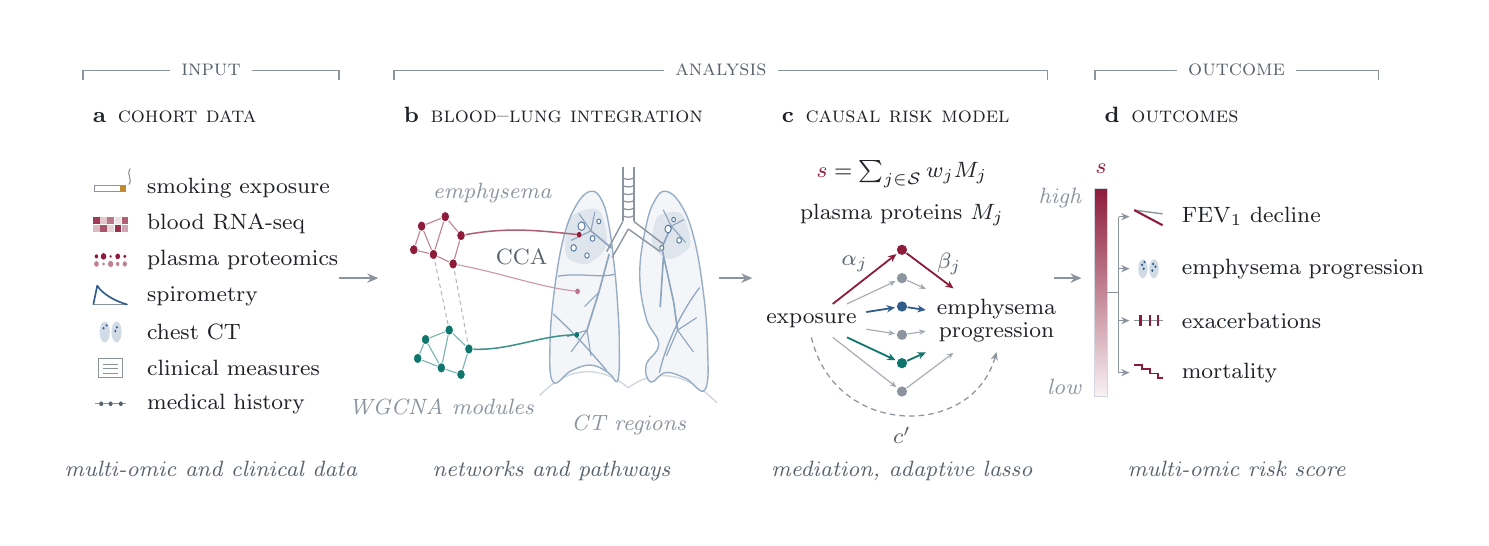
\begin{tikzpicture}[
    yscale=1.2,
    font=\footnotesize, text=ink,
    show background rectangle,
    background rectangle/.style={fill=white},
    inner frame sep=10pt,
    title/.style={anchor=base west, font=\footnotesize},
    sub/.style={anchor=base, text=mute, font=\footnotesize\itshape},
    tag/.style={anchor=north, text=faint, font=\footnotesize\itshape},
    flow/.style={draw=faint, line width=0.6pt, -{Stealth[length=4pt, width=3.4pt]}},
    group/.style={draw=faint, line width=0.5pt},
    grouplabel/.style={text=mute, font=\footnotesize\scshape, fill=white, inner xsep=4pt},
    airway/.style={draw=slate!55, line cap=round},
    path/.style={line width=0.65pt, -{Stealth[length=3pt, width=2.6pt]}, shorten >=0.5pt},
    weak/.style={draw=faint!80, line width=0.4pt, -{Stealth[length=2.4pt, width=2pt]}, shorten >=0.5pt}]

  % ---------------------------------------------------------- titles
  \node[title] at (-0.35,4.05) {\textbf{a}\enspace\textsc{cohort data}};
  \node[title] at (3.60,4.05)  {\textbf{b}\enspace\textsc{blood--lung integration}};
  \node[title] at (8.40,4.05)  {\textbf{c}\enspace\textsc{causal risk model}};
  \node[title] at (12.50,4.05) {\textbf{d}\enspace\textsc{outcomes}};
  \draw[group] (-0.35,4.50) -- ++(0,0.10) -| (2.90,4.50);
  \node[grouplabel] at (1.275,4.60) {input};
  \draw[group] (3.60,4.50) -- ++(0,0.10) -| (11.90,4.50);
  \node[grouplabel] at (7.75,4.60) {analysis};
  \draw[group] (12.50,4.50) -- ++(0,0.10) -| (16.10,4.50);
  \node[grouplabel] at (14.30,4.60) {outcome};

  % --------------------------------------------------- a: cohort data
  \begin{scope}[shift={(0,3.35)}]                                   % smoking
    \fill[white, draw=faint, line width=0.4pt] (-0.20,-0.035) rectangle (0.12,0.035);
    \fill[ochre] (0.12,-0.035) rectangle (0.20,0.035);
    \draw[faint, line width=0.4pt] (0.23,0.04) .. controls (0.29,0.10) and (0.19,0.14) .. (0.25,0.21);
  \end{scope}
  \begin{scope}[shift={(0,2.97)}]                                   % RNA-seq
    \foreach \i/\o in {0/0.85, 1/0.25, 2/0.60, 3/0.15, 4/0.70}
      \fill[risk, opacity=\o] (-0.22+0.09*\i,0.005) rectangle ++(0.08,0.075);
    \foreach \i/\o in {0/0.30, 1/0.75, 2/0.20, 3/0.90, 4/0.40}
      \fill[risk, opacity=\o] (-0.22+0.09*\i,-0.08) rectangle ++(0.08,0.075);
  \end{scope}
  \begin{scope}[shift={(0,2.59)}]                                   % proteomics
    \foreach \i/\r/\s in {0/0.022/0.030, 1/0.035/0.018, 2/0.015/0.034, 3/0.030/0.022, 4/0.020/0.028} {
      \fill[risk] (-0.18+0.09*\i,0.04) circle (\r);
      \fill[risk!55] (-0.18+0.09*\i,-0.04) circle (\s);
    }
  \end{scope}
  \begin{scope}[shift={(0,2.21)}]                                   % spirometry
    \draw[faint, line width=0.3pt] (-0.22,-0.09) -- (0.22,-0.09);
    \draw[slate, line width=0.6pt, line join=round] (-0.22,-0.09) -- (-0.17,0.11)
      .. controls (-0.10,0.02) and (0.05,-0.05) .. (0.21,-0.09);
  \end{scope}
  \begin{scope}[shift={(0,1.83)}]                                   % chest CT
    \fill[slate!22] (-0.075,0) ellipse[x radius=0.065, y radius=0.11];
    \fill[slate!22] (0.075,0) ellipse[x radius=0.065, y radius=0.11];
    \foreach \p in {(-0.09,0.04), (-0.05,0.07), (0.08,0.05), (0.06,0.01)}
      \fill[slate] \p circle (0.014);
  \end{scope}
  \begin{scope}[shift={(0,1.45)}]                                   % clinical measures
    \draw[faint, line width=0.4pt] (-0.15,-0.10) rectangle (0.15,0.10);
    \foreach \y in {0.04,-0.01,-0.06}
      \draw[faint, line width=0.4pt] (-0.10,\y) -- (0.10,\y);
  \end{scope}
  \begin{scope}[shift={(0,1.07)}]                                   % medical history
    \draw[faint, line width=0.45pt] (-0.20,0) -- (0.20,0);
    \foreach \x in {-0.12,0.00,0.13} \fill[mute] (\x,0) circle (0.025);
  \end{scope}
  \foreach \y/\t in {3.35/smoking exposure, 2.97/blood RNA-seq, 2.59/plasma proteomics,
      2.21/spirometry, 1.83/chest CT, 1.45/clinical measures, 1.07/medical history}
    \node[anchor=west] at (0.34,\y) {\t};

  % ------------------------------------------ b: blood-lung integration
  \coordinate (A1) at (3.95,2.95); \coordinate (A2) at (4.25,3.05); \coordinate (A3) at (4.45,2.85);
  \coordinate (A4) at (4.10,2.65); \coordinate (A5) at (4.35,2.55); \coordinate (A6) at (3.85,2.70);
  \coordinate (B1) at (4.00,1.75); \coordinate (B2) at (4.30,1.85); \coordinate (B3) at (4.55,1.65);
  \coordinate (B4) at (4.20,1.45); \coordinate (B5) at (3.90,1.55); \coordinate (B6) at (4.45,1.38);
  \draw[risk!55, line width=0.4pt] (A1)--(A2) (A2)--(A3) (A1)--(A4) (A4)--(A5) (A3)--(A5)
    (A6)--(A1) (A6)--(A4) (A2)--(A4);
  \draw[ml!55, line width=0.4pt] (B1)--(B2) (B2)--(B3) (B1)--(B5) (B5)--(B4) (B4)--(B6)
    (B3)--(B6) (B2)--(B4) (B1)--(B4);
  \draw[faint!70, line width=0.35pt, dash pattern=on 1.5pt off 1.2pt] (A4)--(B2) (A5)--(B3);

  % lungs in anterior view, so the patient's right lung is on the left
  \draw[rule, line width=0.5pt] (5.45,1.16) .. controls (5.85,1.50) and (6.25,1.46) .. (6.575,1.24)
    .. controls (6.90,1.44) and (7.30,1.42) .. (7.70,1.08);                         % diaphragm
  \filldraw[fill=slate!6, draw=slate!50, line width=0.5pt] plot[smooth cycle, tension=0.7] coordinates
    {(6.10,3.32) (5.92,3.18) (5.76,2.85) (5.64,2.30) (5.58,1.70) (5.62,1.30) (5.85,1.42) (6.10,1.48)
     (6.32,1.40) (6.44,1.32) (6.46,1.70) (6.44,2.10) (6.40,2.50) (6.33,2.95) (6.24,3.22)};
  \filldraw[fill=slate!6, draw=slate!50, line width=0.5pt] plot[smooth cycle, tension=0.7] coordinates
    {(7.05,3.32) (7.24,3.18) (7.40,2.85) (7.52,2.30) (7.58,1.70) (7.55,1.22) (7.30,1.34) (7.05,1.40)
     (6.86,1.30) (6.80,1.48) (6.96,1.70) (6.80,1.98) (6.72,2.45) (6.80,2.95) (6.91,3.22)};
  \fill[slate, opacity=0.10] plot[smooth cycle] coordinates                         % upper-lobe emphysema
    {(5.85,3.05) (6.20,3.12) (6.30,2.75) (6.05,2.55) (5.78,2.65)};
  \fill[slate, opacity=0.10] plot[smooth cycle] coordinates
    {(6.95,3.05) (7.25,3.08) (7.36,2.75) (7.10,2.60) (6.88,2.75)};
  \draw[slate!55, line width=0.45pt] (5.68,2.42) .. controls (5.95,2.46) and (6.20,2.40) .. (6.40,2.44);  % horizontal fissure
  \draw[slate!55, line width=0.45pt] (5.62,2.02) .. controls (5.85,1.85) and (6.10,1.62) .. (6.30,1.42);  % right oblique fissure
  \draw[slate!55, line width=0.45pt] (7.48,2.30) .. controls (7.25,2.05) and (7.05,1.70) .. (6.97,1.40);  % left oblique fissure
  \draw[airway, line width=0.6pt] (6.36,2.72) -- (6.10,2.90)  (6.33,2.65) -- (6.20,2.25) -- (6.05,1.85)
    (7.00,2.72) -- (7.12,2.95)  (7.00,2.72) -- (7.15,2.15) -- (7.20,1.85)  (7.02,2.62) -- (6.98,2.10);
  \draw[airway, line width=0.4pt] (6.10,2.90) -- (5.95,3.08)  (6.10,2.90) -- (6.15,3.10)  (6.10,2.90) -- (5.85,2.80)
    (6.20,2.25) -- (6.02,2.10)  (6.05,1.85) -- (5.85,1.62)  (6.05,1.85) -- (6.10,1.58)  (6.05,1.85) -- (5.80,1.78)
    (7.12,2.95) -- (7.02,3.12)  (7.12,2.95) -- (7.28,3.02)  (7.12,2.95) -- (7.30,2.78)
    (7.20,1.85) -- (7.40,1.62)  (7.20,1.85) -- (7.06,1.58)  (7.20,1.85) -- (7.44,1.98);
  \foreach \x/\y/\r in {5.98/2.95/0.045, 6.12/2.82/0.030, 5.88/2.72/0.035, 6.20/3.00/0.025, 6.05/2.64/0.028,
      7.08/2.92/0.040, 7.22/2.80/0.030, 7.00/2.72/0.026, 7.15/3.02/0.024}
    \filldraw[fill=white, draw=slate!80, line width=0.35pt] (\x,\y) circle (\r);
  \fill[white] (6.505,3.00) rectangle (6.645,3.58);                                % trachea
  \draw[faint, line width=0.5pt] (6.505,3.58) -- (6.505,3.00) (6.645,3.58) -- (6.645,3.00);
  \foreach \y in {3.06,3.14,...,3.54}
    \draw[faint, line width=0.45pt] (6.505,\y) .. controls (6.55,\y-0.02) and (6.60,\y-0.02) .. (6.645,\y);
  \draw[faint, line width=0.5pt] (6.505,3.00) -- (6.30,2.68) (6.575,2.92) -- (6.37,2.62)
    (6.645,3.00) -- (7.02,2.76) (6.575,2.92) -- (6.98,2.68);                       % main bronchi

  \draw[risk!70, line width=0.55pt] (A3) .. controls (5.05,2.95) and (5.45,2.90) .. (5.95,2.86);
  \draw[risk!45, line width=0.40pt] (A5) .. controls (5.00,2.45) and (5.45,2.30) .. (5.93,2.26);
  \draw[ml!80, line width=0.55pt] (B3) .. controls (5.05,1.62) and (5.45,1.80) .. (5.92,1.80);
  \fill[risk] (5.95,2.86) circle (0.03);
  \fill[risk!60] (5.93,2.26) circle (0.03);
  \fill[ml] (5.92,1.80) circle (0.03);
  \foreach \n in {A1,A2,A3,A4,A5,A6} \fill[risk, draw=white, line width=0.3pt] (\n) circle (0.055);
  \foreach \n in {B1,B2,B3,B4,B5,B6} \fill[ml, draw=white, line width=0.3pt] (\n) circle (0.055);
  \node[text=mute] at (5.22,2.62) {CCA};
  \node[anchor=east, text=faint, font=\footnotesize\itshape] at (5.72,3.30) {emphysema};
  \node[tag] at (4.20,1.22) {WGCNA modules};
  \node[tag] at (6.58,1.05) {CT regions};

  % ---------------------------------------------- c: causal risk model
  \begin{scope}[shift={(8.50,1.05)}]
    \node (X) at (0.40,0.90) {exposure};
    \node[align=center] (Y) at (2.75,0.90) {emphysema\\[-1pt]progression};
    \foreach \n/\y/\c in {m1/1.65/risk, m2/1.35/faint, m3/1.05/slate, m4/0.75/faint, m5/0.45/ml, m6/0.15/faint}
      \node[circle, fill=\c, inner sep=0pt, minimum size=0.13cm] (\n) at (1.55,\y) {};
    \foreach \n in {m2,m4,m6} {
      \draw[weak] (X) -- (\n);
      \draw[weak] (\n) -- (Y);
    }
    \foreach \n/\c in {m1/risk, m3/slate, m5/ml} {
      \draw[path, draw=\c] (X) -- (\n);
      \draw[path, draw=\c] (\n) -- (Y);
    }
    \draw[faint, line width=0.45pt, dash pattern=on 2pt off 1.5pt, -{Stealth[length=3pt, width=2.6pt]}]
      (X.south) .. controls (0.70,-0.35) and (2.45,-0.35) .. (Y.south);
    \node[anchor=north, text=mute] at (1.55,-0.12) {$c'$};
    \node[text=mute] at (0.95,1.50) {$\alpha_j$};
    \node[text=mute] at (2.15,1.50) {$\beta_j$};
    \node[anchor=south] at (1.55,1.80) {plasma proteins $M_j$};
    \node at (1.55,2.45) {$\textcolor{risk}{s} = \textstyle\sum_{j \in \mathcal{S}} w_j M_j$};
  \end{scope}

  % ------------------------------------------------------ d: outcomes
  \begin{scope}[shift={(12.50,1.00)}]
    \shade[bottom color=risk!6, top color=risk] (0,0.15) rectangle (0.16,2.35);
    \draw[rule, line width=0.4pt] (0,0.15) rectangle (0.16,2.35);
    \node[anchor=south, text=risk] at (0.08,2.40) {$s$};
    \node[anchor=east, text=faint, font=\footnotesize\itshape] at (-0.05,2.25) {high};
    \node[anchor=east, text=faint, font=\footnotesize\itshape] at (-0.05,0.25) {low};
    \draw[faint, line width=0.45pt] (0.16,1.25) -- (0.30,1.25) (0.30,0.40) -- (0.30,2.05);
    \foreach \y in {2.05,1.50,0.95,0.40}
      \draw[faint, line width=0.45pt, -{Stealth[length=3pt, width=2.6pt]}] (0.30,\y) -- (0.44,\y);
    \begin{scope}[shift={(0.68,2.05)}]                              % FEV1 decline
      \draw[faint, line width=0.5pt] (-0.18,0.07) -- (0.18,0.03);
      \draw[risk, line width=0.75pt] (-0.18,0.07) -- (0.18,-0.09);
    \end{scope}
    \begin{scope}[shift={(0.68,1.50)}]                              % emphysema
      \fill[slate!22] (-0.07,0) ellipse[x radius=0.06, y radius=0.10];
      \fill[slate!22] (0.07,0) ellipse[x radius=0.06, y radius=0.10];
      \foreach \p in {(-0.08,0.04), (-0.05,0.07), (-0.06,0.00), (0.06,0.05), (0.09,0.02), (0.05,-0.02)}
        \fill[slate] \p circle (0.015);
    \end{scope}
    \begin{scope}[shift={(0.68,0.95)}]                              % exacerbations
      \draw[faint, line width=0.45pt] (-0.18,0) -- (0.18,0);
      \foreach \x in {-0.10,0.02,0.12} \draw[risk, line width=0.9pt] (\x,-0.06) -- (\x,0.06);
    \end{scope}
    \begin{scope}[shift={(0.68,0.40)}]                              % mortality
      \draw[risk, line width=0.6pt] (-0.18,0.08) -| (-0.08,0.04) -| (0.02,-0.01) -| (0.12,-0.06) -- (0.18,-0.06);
    \end{scope}
    \foreach \y/\t in {2.05/FEV$_1$ decline, 1.50/emphysema progression, 0.95/exacerbations, 0.40/mortality}
      \node[anchor=west] at (0.98,\y) {\t};
  \end{scope}

  % --------------------------------------------------- panel notes
  \node[sub] at (1.27,0.30)  {multi-omic and clinical data};
  \node[sub] at (5.60,0.30)  {networks and pathways};
  \node[sub] at (10.05,0.30) {mediation, adaptive lasso};
  \node[sub] at (14.30,0.30) {multi-omic risk score};

  \draw[flow] (2.90,2.40) -- (3.40,2.40);
  \draw[flow] (7.72,2.40) -- (8.15,2.40);
  \draw[flow] (11.98,2.40) -- (12.33,2.40);
\end{tikzpicture}
\end{document}
"
%          dvisvgm --no-fonts --exact-bbox --optimize research_copd.dvi
\documentclass[tikz,border=0pt]{standalone}
\usepackage[T1]{fontenc}
\usepackage{lmodern}
\usepackage{amsmath}
\usetikzlibrary{arrows.meta,backgrounds}

\definecolor{ink}{HTML}{1F2328}
\definecolor{mute}{HTML}{59636E}
\definecolor{faint}{HTML}{8C959F}
\definecolor{rule}{HTML}{D0D7DE}
\definecolor{risk}{HTML}{8E1B3A}
\definecolor{ochre}{HTML}{C08A2E}
\definecolor{slate}{HTML}{2F5C8A}
\definecolor{ml}{HTML}{0F766E}

\begin{document}
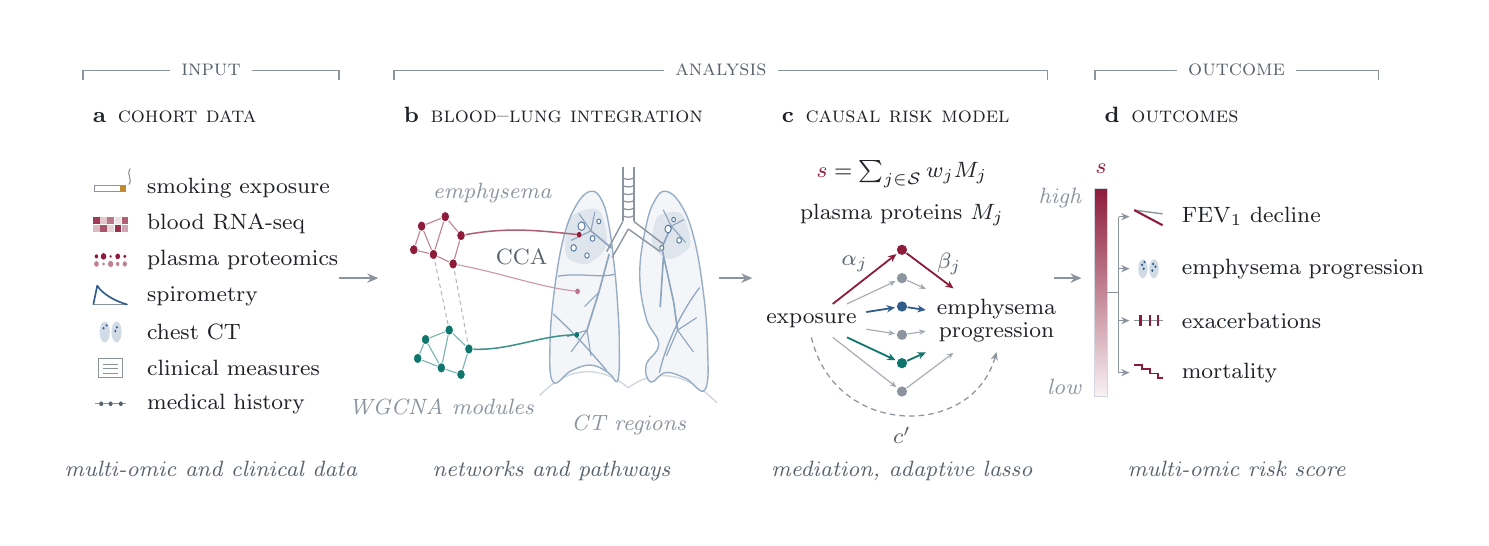
\begin{tikzpicture}[
    yscale=1.2,
    font=\footnotesize, text=ink,
    show background rectangle,
    background rectangle/.style={fill=white},
    inner frame sep=10pt,
    title/.style={anchor=base west, font=\footnotesize},
    sub/.style={anchor=base, text=mute, font=\footnotesize\itshape},
    tag/.style={anchor=north, text=faint, font=\footnotesize\itshape},
    flow/.style={draw=faint, line width=0.6pt, -{Stealth[length=4pt, width=3.4pt]}},
    group/.style={draw=faint, line width=0.5pt},
    grouplabel/.style={text=mute, font=\footnotesize\scshape, fill=white, inner xsep=4pt},
    airway/.style={draw=slate!55, line cap=round},
    path/.style={line width=0.65pt, -{Stealth[length=3pt, width=2.6pt]}, shorten >=0.5pt},
    weak/.style={draw=faint!80, line width=0.4pt, -{Stealth[length=2.4pt, width=2pt]}, shorten >=0.5pt}]

  % ---------------------------------------------------------- titles
  \node[title] at (-0.35,4.05) {\textbf{a}\enspace\textsc{cohort data}};
  \node[title] at (3.60,4.05)  {\textbf{b}\enspace\textsc{blood--lung integration}};
  \node[title] at (8.40,4.05)  {\textbf{c}\enspace\textsc{causal risk model}};
  \node[title] at (12.50,4.05) {\textbf{d}\enspace\textsc{outcomes}};
  \draw[group] (-0.35,4.50) -- ++(0,0.10) -| (2.90,4.50);
  \node[grouplabel] at (1.275,4.60) {input};
  \draw[group] (3.60,4.50) -- ++(0,0.10) -| (11.90,4.50);
  \node[grouplabel] at (7.75,4.60) {analysis};
  \draw[group] (12.50,4.50) -- ++(0,0.10) -| (16.10,4.50);
  \node[grouplabel] at (14.30,4.60) {outcome};

  % --------------------------------------------------- a: cohort data
  \begin{scope}[shift={(0,3.35)}]                                   % smoking
    \fill[white, draw=faint, line width=0.4pt] (-0.20,-0.035) rectangle (0.12,0.035);
    \fill[ochre] (0.12,-0.035) rectangle (0.20,0.035);
    \draw[faint, line width=0.4pt] (0.23,0.04) .. controls (0.29,0.10) and (0.19,0.14) .. (0.25,0.21);
  \end{scope}
  \begin{scope}[shift={(0,2.97)}]                                   % RNA-seq
    \foreach \i/\o in {0/0.85, 1/0.25, 2/0.60, 3/0.15, 4/0.70}
      \fill[risk, opacity=\o] (-0.22+0.09*\i,0.005) rectangle ++(0.08,0.075);
    \foreach \i/\o in {0/0.30, 1/0.75, 2/0.20, 3/0.90, 4/0.40}
      \fill[risk, opacity=\o] (-0.22+0.09*\i,-0.08) rectangle ++(0.08,0.075);
  \end{scope}
  \begin{scope}[shift={(0,2.59)}]                                   % proteomics
    \foreach \i/\r/\s in {0/0.022/0.030, 1/0.035/0.018, 2/0.015/0.034, 3/0.030/0.022, 4/0.020/0.028} {
      \fill[risk] (-0.18+0.09*\i,0.04) circle (\r);
      \fill[risk!55] (-0.18+0.09*\i,-0.04) circle (\s);
    }
  \end{scope}
  \begin{scope}[shift={(0,2.21)}]                                   % spirometry
    \draw[faint, line width=0.3pt] (-0.22,-0.09) -- (0.22,-0.09);
    \draw[slate, line width=0.6pt, line join=round] (-0.22,-0.09) -- (-0.17,0.11)
      .. controls (-0.10,0.02) and (0.05,-0.05) .. (0.21,-0.09);
  \end{scope}
  \begin{scope}[shift={(0,1.83)}]                                   % chest CT
    \fill[slate!22] (-0.075,0) ellipse[x radius=0.065, y radius=0.11];
    \fill[slate!22] (0.075,0) ellipse[x radius=0.065, y radius=0.11];
    \foreach \p in {(-0.09,0.04), (-0.05,0.07), (0.08,0.05), (0.06,0.01)}
      \fill[slate] \p circle (0.014);
  \end{scope}
  \begin{scope}[shift={(0,1.45)}]                                   % clinical measures
    \draw[faint, line width=0.4pt] (-0.15,-0.10) rectangle (0.15,0.10);
    \foreach \y in {0.04,-0.01,-0.06}
      \draw[faint, line width=0.4pt] (-0.10,\y) -- (0.10,\y);
  \end{scope}
  \begin{scope}[shift={(0,1.07)}]                                   % medical history
    \draw[faint, line width=0.45pt] (-0.20,0) -- (0.20,0);
    \foreach \x in {-0.12,0.00,0.13} \fill[mute] (\x,0) circle (0.025);
  \end{scope}
  \foreach \y/\t in {3.35/smoking exposure, 2.97/blood RNA-seq, 2.59/plasma proteomics,
      2.21/spirometry, 1.83/chest CT, 1.45/clinical measures, 1.07/medical history}
    \node[anchor=west] at (0.34,\y) {\t};

  % ------------------------------------------ b: blood-lung integration
  \coordinate (A1) at (3.95,2.95); \coordinate (A2) at (4.25,3.05); \coordinate (A3) at (4.45,2.85);
  \coordinate (A4) at (4.10,2.65); \coordinate (A5) at (4.35,2.55); \coordinate (A6) at (3.85,2.70);
  \coordinate (B1) at (4.00,1.75); \coordinate (B2) at (4.30,1.85); \coordinate (B3) at (4.55,1.65);
  \coordinate (B4) at (4.20,1.45); \coordinate (B5) at (3.90,1.55); \coordinate (B6) at (4.45,1.38);
  \draw[risk!55, line width=0.4pt] (A1)--(A2) (A2)--(A3) (A1)--(A4) (A4)--(A5) (A3)--(A5)
    (A6)--(A1) (A6)--(A4) (A2)--(A4);
  \draw[ml!55, line width=0.4pt] (B1)--(B2) (B2)--(B3) (B1)--(B5) (B5)--(B4) (B4)--(B6)
    (B3)--(B6) (B2)--(B4) (B1)--(B4);
  \draw[faint!70, line width=0.35pt, dash pattern=on 1.5pt off 1.2pt] (A4)--(B2) (A5)--(B3);

  % lungs in anterior view, so the patient's right lung is on the left
  \draw[rule, line width=0.5pt] (5.45,1.16) .. controls (5.85,1.50) and (6.25,1.46) .. (6.575,1.24)
    .. controls (6.90,1.44) and (7.30,1.42) .. (7.70,1.08);                         % diaphragm
  \filldraw[fill=slate!6, draw=slate!50, line width=0.5pt] plot[smooth cycle, tension=0.7] coordinates
    {(6.10,3.32) (5.92,3.18) (5.76,2.85) (5.64,2.30) (5.58,1.70) (5.62,1.30) (5.85,1.42) (6.10,1.48)
     (6.32,1.40) (6.44,1.32) (6.46,1.70) (6.44,2.10) (6.40,2.50) (6.33,2.95) (6.24,3.22)};
  \filldraw[fill=slate!6, draw=slate!50, line width=0.5pt] plot[smooth cycle, tension=0.7] coordinates
    {(7.05,3.32) (7.24,3.18) (7.40,2.85) (7.52,2.30) (7.58,1.70) (7.55,1.22) (7.30,1.34) (7.05,1.40)
     (6.86,1.30) (6.80,1.48) (6.96,1.70) (6.80,1.98) (6.72,2.45) (6.80,2.95) (6.91,3.22)};
  \fill[slate, opacity=0.10] plot[smooth cycle] coordinates                         % upper-lobe emphysema
    {(5.85,3.05) (6.20,3.12) (6.30,2.75) (6.05,2.55) (5.78,2.65)};
  \fill[slate, opacity=0.10] plot[smooth cycle] coordinates
    {(6.95,3.05) (7.25,3.08) (7.36,2.75) (7.10,2.60) (6.88,2.75)};
  \draw[slate!55, line width=0.45pt] (5.68,2.42) .. controls (5.95,2.46) and (6.20,2.40) .. (6.40,2.44);  % horizontal fissure
  \draw[slate!55, line width=0.45pt] (5.62,2.02) .. controls (5.85,1.85) and (6.10,1.62) .. (6.30,1.42);  % right oblique fissure
  \draw[slate!55, line width=0.45pt] (7.48,2.30) .. controls (7.25,2.05) and (7.05,1.70) .. (6.97,1.40);  % left oblique fissure
  \draw[airway, line width=0.6pt] (6.36,2.72) -- (6.10,2.90)  (6.33,2.65) -- (6.20,2.25) -- (6.05,1.85)
    (7.00,2.72) -- (7.12,2.95)  (7.00,2.72) -- (7.15,2.15) -- (7.20,1.85)  (7.02,2.62) -- (6.98,2.10);
  \draw[airway, line width=0.4pt] (6.10,2.90) -- (5.95,3.08)  (6.10,2.90) -- (6.15,3.10)  (6.10,2.90) -- (5.85,2.80)
    (6.20,2.25) -- (6.02,2.10)  (6.05,1.85) -- (5.85,1.62)  (6.05,1.85) -- (6.10,1.58)  (6.05,1.85) -- (5.80,1.78)
    (7.12,2.95) -- (7.02,3.12)  (7.12,2.95) -- (7.28,3.02)  (7.12,2.95) -- (7.30,2.78)
    (7.20,1.85) -- (7.40,1.62)  (7.20,1.85) -- (7.06,1.58)  (7.20,1.85) -- (7.44,1.98);
  \foreach \x/\y/\r in {5.98/2.95/0.045, 6.12/2.82/0.030, 5.88/2.72/0.035, 6.20/3.00/0.025, 6.05/2.64/0.028,
      7.08/2.92/0.040, 7.22/2.80/0.030, 7.00/2.72/0.026, 7.15/3.02/0.024}
    \filldraw[fill=white, draw=slate!80, line width=0.35pt] (\x,\y) circle (\r);
  \fill[white] (6.505,3.00) rectangle (6.645,3.58);                                % trachea
  \draw[faint, line width=0.5pt] (6.505,3.58) -- (6.505,3.00) (6.645,3.58) -- (6.645,3.00);
  \foreach \y in {3.06,3.14,...,3.54}
    \draw[faint, line width=0.45pt] (6.505,\y) .. controls (6.55,\y-0.02) and (6.60,\y-0.02) .. (6.645,\y);
  \draw[faint, line width=0.5pt] (6.505,3.00) -- (6.30,2.68) (6.575,2.92) -- (6.37,2.62)
    (6.645,3.00) -- (7.02,2.76) (6.575,2.92) -- (6.98,2.68);                       % main bronchi

  \draw[risk!70, line width=0.55pt] (A3) .. controls (5.05,2.95) and (5.45,2.90) .. (5.95,2.86);
  \draw[risk!45, line width=0.40pt] (A5) .. controls (5.00,2.45) and (5.45,2.30) .. (5.93,2.26);
  \draw[ml!80, line width=0.55pt] (B3) .. controls (5.05,1.62) and (5.45,1.80) .. (5.92,1.80);
  \fill[risk] (5.95,2.86) circle (0.03);
  \fill[risk!60] (5.93,2.26) circle (0.03);
  \fill[ml] (5.92,1.80) circle (0.03);
  \foreach \n in {A1,A2,A3,A4,A5,A6} \fill[risk, draw=white, line width=0.3pt] (\n) circle (0.055);
  \foreach \n in {B1,B2,B3,B4,B5,B6} \fill[ml, draw=white, line width=0.3pt] (\n) circle (0.055);
  \node[text=mute] at (5.22,2.62) {CCA};
  \node[anchor=east, text=faint, font=\footnotesize\itshape] at (5.72,3.30) {emphysema};
  \node[tag] at (4.20,1.22) {WGCNA modules};
  \node[tag] at (6.58,1.05) {CT regions};

  % ---------------------------------------------- c: causal risk model
  \begin{scope}[shift={(8.50,1.05)}]
    \node (X) at (0.40,0.90) {exposure};
    \node[align=center] (Y) at (2.75,0.90) {emphysema\\[-1pt]progression};
    \foreach \n/\y/\c in {m1/1.65/risk, m2/1.35/faint, m3/1.05/slate, m4/0.75/faint, m5/0.45/ml, m6/0.15/faint}
      \node[circle, fill=\c, inner sep=0pt, minimum size=0.13cm] (\n) at (1.55,\y) {};
    \foreach \n in {m2,m4,m6} {
      \draw[weak] (X) -- (\n);
      \draw[weak] (\n) -- (Y);
    }
    \foreach \n/\c in {m1/risk, m3/slate, m5/ml} {
      \draw[path, draw=\c] (X) -- (\n);
      \draw[path, draw=\c] (\n) -- (Y);
    }
    \draw[faint, line width=0.45pt, dash pattern=on 2pt off 1.5pt, -{Stealth[length=3pt, width=2.6pt]}]
      (X.south) .. controls (0.70,-0.35) and (2.45,-0.35) .. (Y.south);
    \node[anchor=north, text=mute] at (1.55,-0.12) {$c'$};
    \node[text=mute] at (0.95,1.50) {$\alpha_j$};
    \node[text=mute] at (2.15,1.50) {$\beta_j$};
    \node[anchor=south] at (1.55,1.80) {plasma proteins $M_j$};
    \node at (1.55,2.45) {$\textcolor{risk}{s} = \textstyle\sum_{j \in \mathcal{S}} w_j M_j$};
  \end{scope}

  % ------------------------------------------------------ d: outcomes
  \begin{scope}[shift={(12.50,1.00)}]
    \shade[bottom color=risk!6, top color=risk] (0,0.15) rectangle (0.16,2.35);
    \draw[rule, line width=0.4pt] (0,0.15) rectangle (0.16,2.35);
    \node[anchor=south, text=risk] at (0.08,2.40) {$s$};
    \node[anchor=east, text=faint, font=\footnotesize\itshape] at (-0.05,2.25) {high};
    \node[anchor=east, text=faint, font=\footnotesize\itshape] at (-0.05,0.25) {low};
    \draw[faint, line width=0.45pt] (0.16,1.25) -- (0.30,1.25) (0.30,0.40) -- (0.30,2.05);
    \foreach \y in {2.05,1.50,0.95,0.40}
      \draw[faint, line width=0.45pt, -{Stealth[length=3pt, width=2.6pt]}] (0.30,\y) -- (0.44,\y);
    \begin{scope}[shift={(0.68,2.05)}]                              % FEV1 decline
      \draw[faint, line width=0.5pt] (-0.18,0.07) -- (0.18,0.03);
      \draw[risk, line width=0.75pt] (-0.18,0.07) -- (0.18,-0.09);
    \end{scope}
    \begin{scope}[shift={(0.68,1.50)}]                              % emphysema
      \fill[slate!22] (-0.07,0) ellipse[x radius=0.06, y radius=0.10];
      \fill[slate!22] (0.07,0) ellipse[x radius=0.06, y radius=0.10];
      \foreach \p in {(-0.08,0.04), (-0.05,0.07), (-0.06,0.00), (0.06,0.05), (0.09,0.02), (0.05,-0.02)}
        \fill[slate] \p circle (0.015);
    \end{scope}
    \begin{scope}[shift={(0.68,0.95)}]                              % exacerbations
      \draw[faint, line width=0.45pt] (-0.18,0) -- (0.18,0);
      \foreach \x in {-0.10,0.02,0.12} \draw[risk, line width=0.9pt] (\x,-0.06) -- (\x,0.06);
    \end{scope}
    \begin{scope}[shift={(0.68,0.40)}]                              % mortality
      \draw[risk, line width=0.6pt] (-0.18,0.08) -| (-0.08,0.04) -| (0.02,-0.01) -| (0.12,-0.06) -- (0.18,-0.06);
    \end{scope}
    \foreach \y/\t in {2.05/FEV$_1$ decline, 1.50/emphysema progression, 0.95/exacerbations, 0.40/mortality}
      \node[anchor=west] at (0.98,\y) {\t};
  \end{scope}

  % --------------------------------------------------- panel notes
  \node[sub] at (1.27,0.30)  {multi-omic and clinical data};
  \node[sub] at (5.60,0.30)  {networks and pathways};
  \node[sub] at (10.05,0.30) {mediation, adaptive lasso};
  \node[sub] at (14.30,0.30) {multi-omic risk score};

  \draw[flow] (2.90,2.40) -- (3.40,2.40);
  \draw[flow] (7.72,2.40) -- (8.15,2.40);
  \draw[flow] (11.98,2.40) -- (12.33,2.40);
\end{tikzpicture}
\end{document}
"
%          dvisvgm --no-fonts --exact-bbox --optimize research_copd.dvi
\documentclass[tikz,border=0pt]{standalone}
\usepackage[T1]{fontenc}
\usepackage{lmodern}
\usepackage{amsmath}
\usetikzlibrary{arrows.meta,backgrounds}

\definecolor{ink}{HTML}{1F2328}
\definecolor{mute}{HTML}{59636E}
\definecolor{faint}{HTML}{8C959F}
\definecolor{rule}{HTML}{D0D7DE}
\definecolor{risk}{HTML}{8E1B3A}
\definecolor{ochre}{HTML}{C08A2E}
\definecolor{slate}{HTML}{2F5C8A}
\definecolor{ml}{HTML}{0F766E}

\begin{document}
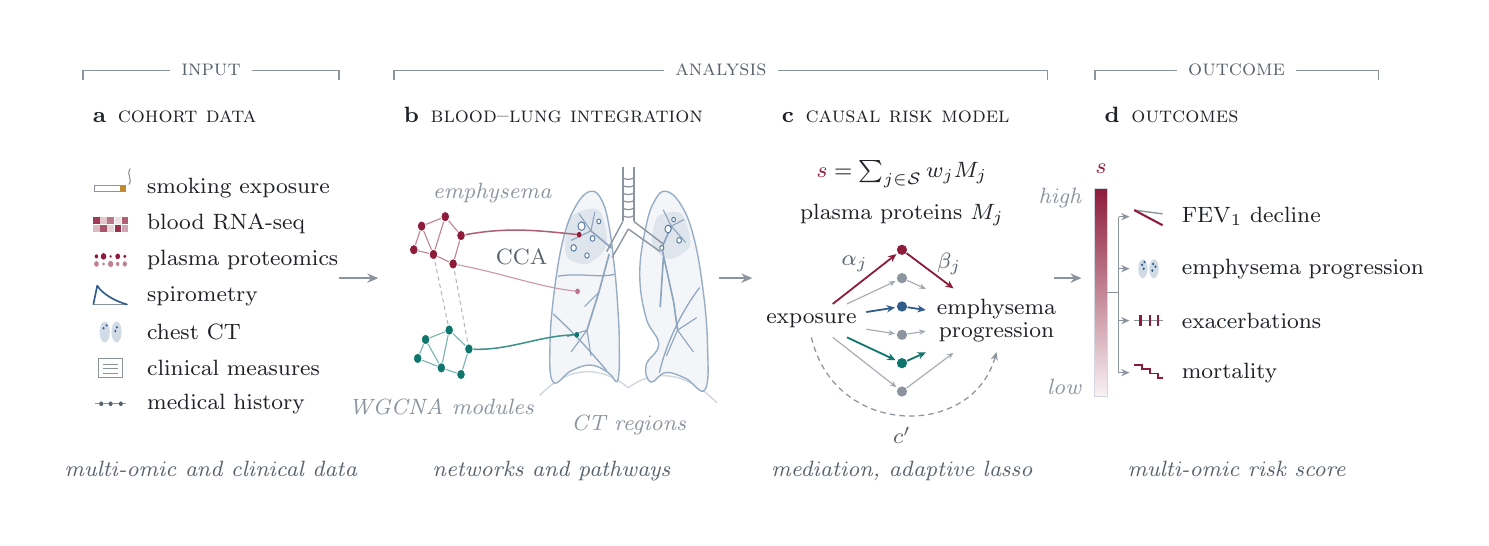
\begin{tikzpicture}[
    yscale=1.2,
    font=\footnotesize, text=ink,
    show background rectangle,
    background rectangle/.style={fill=white},
    inner frame sep=10pt,
    title/.style={anchor=base west, font=\footnotesize},
    sub/.style={anchor=base, text=mute, font=\footnotesize\itshape},
    tag/.style={anchor=north, text=faint, font=\footnotesize\itshape},
    flow/.style={draw=faint, line width=0.6pt, -{Stealth[length=4pt, width=3.4pt]}},
    group/.style={draw=faint, line width=0.5pt},
    grouplabel/.style={text=mute, font=\footnotesize\scshape, fill=white, inner xsep=4pt},
    airway/.style={draw=slate!55, line cap=round},
    path/.style={line width=0.65pt, -{Stealth[length=3pt, width=2.6pt]}, shorten >=0.5pt},
    weak/.style={draw=faint!80, line width=0.4pt, -{Stealth[length=2.4pt, width=2pt]}, shorten >=0.5pt}]

  % ---------------------------------------------------------- titles
  \node[title] at (-0.35,4.05) {\textbf{a}\enspace\textsc{cohort data}};
  \node[title] at (3.60,4.05)  {\textbf{b}\enspace\textsc{blood--lung integration}};
  \node[title] at (8.40,4.05)  {\textbf{c}\enspace\textsc{causal risk model}};
  \node[title] at (12.50,4.05) {\textbf{d}\enspace\textsc{outcomes}};
  \draw[group] (-0.35,4.50) -- ++(0,0.10) -| (2.90,4.50);
  \node[grouplabel] at (1.275,4.60) {input};
  \draw[group] (3.60,4.50) -- ++(0,0.10) -| (11.90,4.50);
  \node[grouplabel] at (7.75,4.60) {analysis};
  \draw[group] (12.50,4.50) -- ++(0,0.10) -| (16.10,4.50);
  \node[grouplabel] at (14.30,4.60) {outcome};

  % --------------------------------------------------- a: cohort data
  \begin{scope}[shift={(0,3.35)}]                                   % smoking
    \fill[white, draw=faint, line width=0.4pt] (-0.20,-0.035) rectangle (0.12,0.035);
    \fill[ochre] (0.12,-0.035) rectangle (0.20,0.035);
    \draw[faint, line width=0.4pt] (0.23,0.04) .. controls (0.29,0.10) and (0.19,0.14) .. (0.25,0.21);
  \end{scope}
  \begin{scope}[shift={(0,2.97)}]                                   % RNA-seq
    \foreach \i/\o in {0/0.85, 1/0.25, 2/0.60, 3/0.15, 4/0.70}
      \fill[risk, opacity=\o] (-0.22+0.09*\i,0.005) rectangle ++(0.08,0.075);
    \foreach \i/\o in {0/0.30, 1/0.75, 2/0.20, 3/0.90, 4/0.40}
      \fill[risk, opacity=\o] (-0.22+0.09*\i,-0.08) rectangle ++(0.08,0.075);
  \end{scope}
  \begin{scope}[shift={(0,2.59)}]                                   % proteomics
    \foreach \i/\r/\s in {0/0.022/0.030, 1/0.035/0.018, 2/0.015/0.034, 3/0.030/0.022, 4/0.020/0.028} {
      \fill[risk] (-0.18+0.09*\i,0.04) circle (\r);
      \fill[risk!55] (-0.18+0.09*\i,-0.04) circle (\s);
    }
  \end{scope}
  \begin{scope}[shift={(0,2.21)}]                                   % spirometry
    \draw[faint, line width=0.3pt] (-0.22,-0.09) -- (0.22,-0.09);
    \draw[slate, line width=0.6pt, line join=round] (-0.22,-0.09) -- (-0.17,0.11)
      .. controls (-0.10,0.02) and (0.05,-0.05) .. (0.21,-0.09);
  \end{scope}
  \begin{scope}[shift={(0,1.83)}]                                   % chest CT
    \fill[slate!22] (-0.075,0) ellipse[x radius=0.065, y radius=0.11];
    \fill[slate!22] (0.075,0) ellipse[x radius=0.065, y radius=0.11];
    \foreach \p in {(-0.09,0.04), (-0.05,0.07), (0.08,0.05), (0.06,0.01)}
      \fill[slate] \p circle (0.014);
  \end{scope}
  \begin{scope}[shift={(0,1.45)}]                                   % clinical measures
    \draw[faint, line width=0.4pt] (-0.15,-0.10) rectangle (0.15,0.10);
    \foreach \y in {0.04,-0.01,-0.06}
      \draw[faint, line width=0.4pt] (-0.10,\y) -- (0.10,\y);
  \end{scope}
  \begin{scope}[shift={(0,1.07)}]                                   % medical history
    \draw[faint, line width=0.45pt] (-0.20,0) -- (0.20,0);
    \foreach \x in {-0.12,0.00,0.13} \fill[mute] (\x,0) circle (0.025);
  \end{scope}
  \foreach \y/\t in {3.35/smoking exposure, 2.97/blood RNA-seq, 2.59/plasma proteomics,
      2.21/spirometry, 1.83/chest CT, 1.45/clinical measures, 1.07/medical history}
    \node[anchor=west] at (0.34,\y) {\t};

  % ------------------------------------------ b: blood-lung integration
  \coordinate (A1) at (3.95,2.95); \coordinate (A2) at (4.25,3.05); \coordinate (A3) at (4.45,2.85);
  \coordinate (A4) at (4.10,2.65); \coordinate (A5) at (4.35,2.55); \coordinate (A6) at (3.85,2.70);
  \coordinate (B1) at (4.00,1.75); \coordinate (B2) at (4.30,1.85); \coordinate (B3) at (4.55,1.65);
  \coordinate (B4) at (4.20,1.45); \coordinate (B5) at (3.90,1.55); \coordinate (B6) at (4.45,1.38);
  \draw[risk!55, line width=0.4pt] (A1)--(A2) (A2)--(A3) (A1)--(A4) (A4)--(A5) (A3)--(A5)
    (A6)--(A1) (A6)--(A4) (A2)--(A4);
  \draw[ml!55, line width=0.4pt] (B1)--(B2) (B2)--(B3) (B1)--(B5) (B5)--(B4) (B4)--(B6)
    (B3)--(B6) (B2)--(B4) (B1)--(B4);
  \draw[faint!70, line width=0.35pt, dash pattern=on 1.5pt off 1.2pt] (A4)--(B2) (A5)--(B3);

  % lungs in anterior view, so the patient's right lung is on the left
  \draw[rule, line width=0.5pt] (5.45,1.16) .. controls (5.85,1.50) and (6.25,1.46) .. (6.575,1.24)
    .. controls (6.90,1.44) and (7.30,1.42) .. (7.70,1.08);                         % diaphragm
  \filldraw[fill=slate!6, draw=slate!50, line width=0.5pt] plot[smooth cycle, tension=0.7] coordinates
    {(6.10,3.32) (5.92,3.18) (5.76,2.85) (5.64,2.30) (5.58,1.70) (5.62,1.30) (5.85,1.42) (6.10,1.48)
     (6.32,1.40) (6.44,1.32) (6.46,1.70) (6.44,2.10) (6.40,2.50) (6.33,2.95) (6.24,3.22)};
  \filldraw[fill=slate!6, draw=slate!50, line width=0.5pt] plot[smooth cycle, tension=0.7] coordinates
    {(7.05,3.32) (7.24,3.18) (7.40,2.85) (7.52,2.30) (7.58,1.70) (7.55,1.22) (7.30,1.34) (7.05,1.40)
     (6.86,1.30) (6.80,1.48) (6.96,1.70) (6.80,1.98) (6.72,2.45) (6.80,2.95) (6.91,3.22)};
  \fill[slate, opacity=0.10] plot[smooth cycle] coordinates                         % upper-lobe emphysema
    {(5.85,3.05) (6.20,3.12) (6.30,2.75) (6.05,2.55) (5.78,2.65)};
  \fill[slate, opacity=0.10] plot[smooth cycle] coordinates
    {(6.95,3.05) (7.25,3.08) (7.36,2.75) (7.10,2.60) (6.88,2.75)};
  \draw[slate!55, line width=0.45pt] (5.68,2.42) .. controls (5.95,2.46) and (6.20,2.40) .. (6.40,2.44);  % horizontal fissure
  \draw[slate!55, line width=0.45pt] (5.62,2.02) .. controls (5.85,1.85) and (6.10,1.62) .. (6.30,1.42);  % right oblique fissure
  \draw[slate!55, line width=0.45pt] (7.48,2.30) .. controls (7.25,2.05) and (7.05,1.70) .. (6.97,1.40);  % left oblique fissure
  \draw[airway, line width=0.6pt] (6.36,2.72) -- (6.10,2.90)  (6.33,2.65) -- (6.20,2.25) -- (6.05,1.85)
    (7.00,2.72) -- (7.12,2.95)  (7.00,2.72) -- (7.15,2.15) -- (7.20,1.85)  (7.02,2.62) -- (6.98,2.10);
  \draw[airway, line width=0.4pt] (6.10,2.90) -- (5.95,3.08)  (6.10,2.90) -- (6.15,3.10)  (6.10,2.90) -- (5.85,2.80)
    (6.20,2.25) -- (6.02,2.10)  (6.05,1.85) -- (5.85,1.62)  (6.05,1.85) -- (6.10,1.58)  (6.05,1.85) -- (5.80,1.78)
    (7.12,2.95) -- (7.02,3.12)  (7.12,2.95) -- (7.28,3.02)  (7.12,2.95) -- (7.30,2.78)
    (7.20,1.85) -- (7.40,1.62)  (7.20,1.85) -- (7.06,1.58)  (7.20,1.85) -- (7.44,1.98);
  \foreach \x/\y/\r in {5.98/2.95/0.045, 6.12/2.82/0.030, 5.88/2.72/0.035, 6.20/3.00/0.025, 6.05/2.64/0.028,
      7.08/2.92/0.040, 7.22/2.80/0.030, 7.00/2.72/0.026, 7.15/3.02/0.024}
    \filldraw[fill=white, draw=slate!80, line width=0.35pt] (\x,\y) circle (\r);
  \fill[white] (6.505,3.00) rectangle (6.645,3.58);                                % trachea
  \draw[faint, line width=0.5pt] (6.505,3.58) -- (6.505,3.00) (6.645,3.58) -- (6.645,3.00);
  \foreach \y in {3.06,3.14,...,3.54}
    \draw[faint, line width=0.45pt] (6.505,\y) .. controls (6.55,\y-0.02) and (6.60,\y-0.02) .. (6.645,\y);
  \draw[faint, line width=0.5pt] (6.505,3.00) -- (6.30,2.68) (6.575,2.92) -- (6.37,2.62)
    (6.645,3.00) -- (7.02,2.76) (6.575,2.92) -- (6.98,2.68);                       % main bronchi

  \draw[risk!70, line width=0.55pt] (A3) .. controls (5.05,2.95) and (5.45,2.90) .. (5.95,2.86);
  \draw[risk!45, line width=0.40pt] (A5) .. controls (5.00,2.45) and (5.45,2.30) .. (5.93,2.26);
  \draw[ml!80, line width=0.55pt] (B3) .. controls (5.05,1.62) and (5.45,1.80) .. (5.92,1.80);
  \fill[risk] (5.95,2.86) circle (0.03);
  \fill[risk!60] (5.93,2.26) circle (0.03);
  \fill[ml] (5.92,1.80) circle (0.03);
  \foreach \n in {A1,A2,A3,A4,A5,A6} \fill[risk, draw=white, line width=0.3pt] (\n) circle (0.055);
  \foreach \n in {B1,B2,B3,B4,B5,B6} \fill[ml, draw=white, line width=0.3pt] (\n) circle (0.055);
  \node[text=mute] at (5.22,2.62) {CCA};
  \node[anchor=east, text=faint, font=\footnotesize\itshape] at (5.72,3.30) {emphysema};
  \node[tag] at (4.20,1.22) {WGCNA modules};
  \node[tag] at (6.58,1.05) {CT regions};

  % ---------------------------------------------- c: causal risk model
  \begin{scope}[shift={(8.50,1.05)}]
    \node (X) at (0.40,0.90) {exposure};
    \node[align=center] (Y) at (2.75,0.90) {emphysema\\[-1pt]progression};
    \foreach \n/\y/\c in {m1/1.65/risk, m2/1.35/faint, m3/1.05/slate, m4/0.75/faint, m5/0.45/ml, m6/0.15/faint}
      \node[circle, fill=\c, inner sep=0pt, minimum size=0.13cm] (\n) at (1.55,\y) {};
    \foreach \n in {m2,m4,m6} {
      \draw[weak] (X) -- (\n);
      \draw[weak] (\n) -- (Y);
    }
    \foreach \n/\c in {m1/risk, m3/slate, m5/ml} {
      \draw[path, draw=\c] (X) -- (\n);
      \draw[path, draw=\c] (\n) -- (Y);
    }
    \draw[faint, line width=0.45pt, dash pattern=on 2pt off 1.5pt, -{Stealth[length=3pt, width=2.6pt]}]
      (X.south) .. controls (0.70,-0.35) and (2.45,-0.35) .. (Y.south);
    \node[anchor=north, text=mute] at (1.55,-0.12) {$c'$};
    \node[text=mute] at (0.95,1.50) {$\alpha_j$};
    \node[text=mute] at (2.15,1.50) {$\beta_j$};
    \node[anchor=south] at (1.55,1.80) {plasma proteins $M_j$};
    \node at (1.55,2.45) {$\textcolor{risk}{s} = \textstyle\sum_{j \in \mathcal{S}} w_j M_j$};
  \end{scope}

  % ------------------------------------------------------ d: outcomes
  \begin{scope}[shift={(12.50,1.00)}]
    \shade[bottom color=risk!6, top color=risk] (0,0.15) rectangle (0.16,2.35);
    \draw[rule, line width=0.4pt] (0,0.15) rectangle (0.16,2.35);
    \node[anchor=south, text=risk] at (0.08,2.40) {$s$};
    \node[anchor=east, text=faint, font=\footnotesize\itshape] at (-0.05,2.25) {high};
    \node[anchor=east, text=faint, font=\footnotesize\itshape] at (-0.05,0.25) {low};
    \draw[faint, line width=0.45pt] (0.16,1.25) -- (0.30,1.25) (0.30,0.40) -- (0.30,2.05);
    \foreach \y in {2.05,1.50,0.95,0.40}
      \draw[faint, line width=0.45pt, -{Stealth[length=3pt, width=2.6pt]}] (0.30,\y) -- (0.44,\y);
    \begin{scope}[shift={(0.68,2.05)}]                              % FEV1 decline
      \draw[faint, line width=0.5pt] (-0.18,0.07) -- (0.18,0.03);
      \draw[risk, line width=0.75pt] (-0.18,0.07) -- (0.18,-0.09);
    \end{scope}
    \begin{scope}[shift={(0.68,1.50)}]                              % emphysema
      \fill[slate!22] (-0.07,0) ellipse[x radius=0.06, y radius=0.10];
      \fill[slate!22] (0.07,0) ellipse[x radius=0.06, y radius=0.10];
      \foreach \p in {(-0.08,0.04), (-0.05,0.07), (-0.06,0.00), (0.06,0.05), (0.09,0.02), (0.05,-0.02)}
        \fill[slate] \p circle (0.015);
    \end{scope}
    \begin{scope}[shift={(0.68,0.95)}]                              % exacerbations
      \draw[faint, line width=0.45pt] (-0.18,0) -- (0.18,0);
      \foreach \x in {-0.10,0.02,0.12} \draw[risk, line width=0.9pt] (\x,-0.06) -- (\x,0.06);
    \end{scope}
    \begin{scope}[shift={(0.68,0.40)}]                              % mortality
      \draw[risk, line width=0.6pt] (-0.18,0.08) -| (-0.08,0.04) -| (0.02,-0.01) -| (0.12,-0.06) -- (0.18,-0.06);
    \end{scope}
    \foreach \y/\t in {2.05/FEV$_1$ decline, 1.50/emphysema progression, 0.95/exacerbations, 0.40/mortality}
      \node[anchor=west] at (0.98,\y) {\t};
  \end{scope}

  % --------------------------------------------------- panel notes
  \node[sub] at (1.27,0.30)  {multi-omic and clinical data};
  \node[sub] at (5.60,0.30)  {networks and pathways};
  \node[sub] at (10.05,0.30) {mediation, adaptive lasso};
  \node[sub] at (14.30,0.30) {multi-omic risk score};

  \draw[flow] (2.90,2.40) -- (3.40,2.40);
  \draw[flow] (7.72,2.40) -- (8.15,2.40);
  \draw[flow] (11.98,2.40) -- (12.33,2.40);
\end{tikzpicture}
\end{document}
"
%          dvisvgm --no-fonts --exact-bbox --optimize research_copd.dvi
\documentclass[tikz,border=0pt]{standalone}
\usepackage[T1]{fontenc}
\usepackage{lmodern}
\usepackage{amsmath}
\usetikzlibrary{arrows.meta,backgrounds}

\definecolor{ink}{HTML}{1F2328}
\definecolor{mute}{HTML}{59636E}
\definecolor{faint}{HTML}{8C959F}
\definecolor{rule}{HTML}{D0D7DE}
\definecolor{risk}{HTML}{8E1B3A}
\definecolor{ochre}{HTML}{C08A2E}
\definecolor{slate}{HTML}{2F5C8A}
\definecolor{ml}{HTML}{0F766E}

\begin{document}
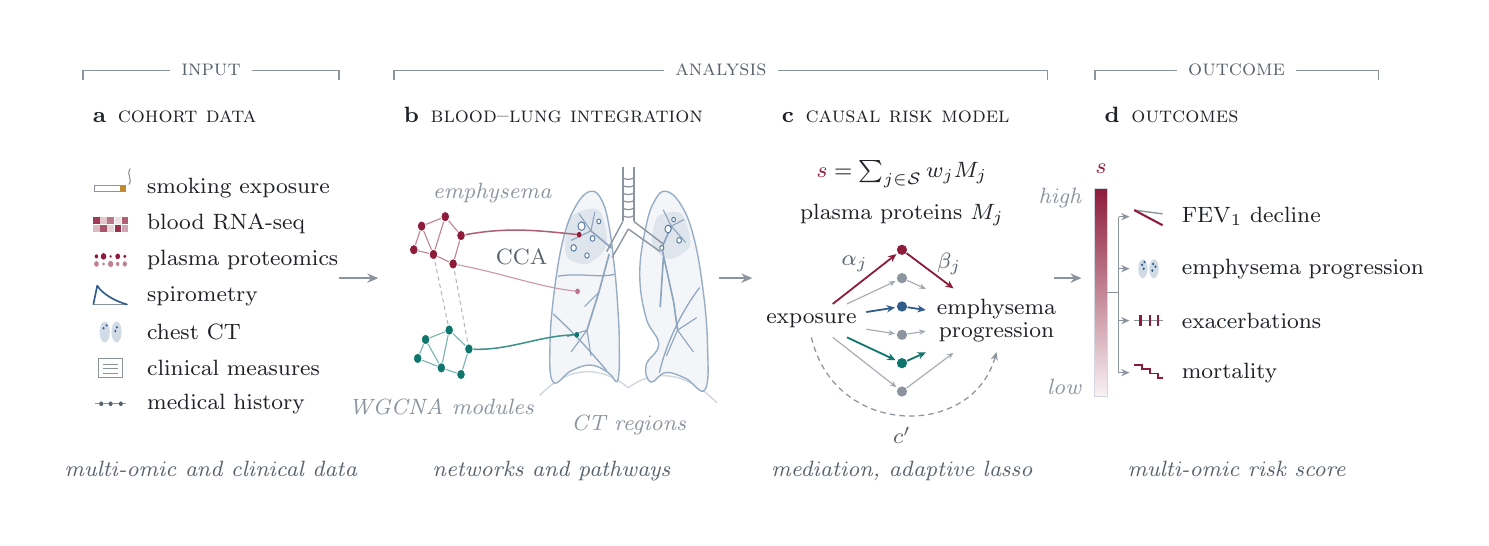
\begin{tikzpicture}[
    yscale=1.2,
    font=\footnotesize, text=ink,
    show background rectangle,
    background rectangle/.style={fill=white},
    inner frame sep=10pt,
    title/.style={anchor=base west, font=\footnotesize},
    sub/.style={anchor=base, text=mute, font=\footnotesize\itshape},
    tag/.style={anchor=north, text=faint, font=\footnotesize\itshape},
    flow/.style={draw=faint, line width=0.6pt, -{Stealth[length=4pt, width=3.4pt]}},
    group/.style={draw=faint, line width=0.5pt},
    grouplabel/.style={text=mute, font=\footnotesize\scshape, fill=white, inner xsep=4pt},
    airway/.style={draw=slate!55, line cap=round},
    path/.style={line width=0.65pt, -{Stealth[length=3pt, width=2.6pt]}, shorten >=0.5pt},
    weak/.style={draw=faint!80, line width=0.4pt, -{Stealth[length=2.4pt, width=2pt]}, shorten >=0.5pt}]

  % ---------------------------------------------------------- titles
  \node[title] at (-0.35,4.05) {\textbf{a}\enspace\textsc{cohort data}};
  \node[title] at (3.60,4.05)  {\textbf{b}\enspace\textsc{blood--lung integration}};
  \node[title] at (8.40,4.05)  {\textbf{c}\enspace\textsc{causal risk model}};
  \node[title] at (12.50,4.05) {\textbf{d}\enspace\textsc{outcomes}};
  \draw[group] (-0.35,4.50) -- ++(0,0.10) -| (2.90,4.50);
  \node[grouplabel] at (1.275,4.60) {input};
  \draw[group] (3.60,4.50) -- ++(0,0.10) -| (11.90,4.50);
  \node[grouplabel] at (7.75,4.60) {analysis};
  \draw[group] (12.50,4.50) -- ++(0,0.10) -| (16.10,4.50);
  \node[grouplabel] at (14.30,4.60) {outcome};

  % --------------------------------------------------- a: cohort data
  \begin{scope}[shift={(0,3.35)}]                                   % smoking
    \fill[white, draw=faint, line width=0.4pt] (-0.20,-0.035) rectangle (0.12,0.035);
    \fill[ochre] (0.12,-0.035) rectangle (0.20,0.035);
    \draw[faint, line width=0.4pt] (0.23,0.04) .. controls (0.29,0.10) and (0.19,0.14) .. (0.25,0.21);
  \end{scope}
  \begin{scope}[shift={(0,2.97)}]                                   % RNA-seq
    \foreach \i/\o in {0/0.85, 1/0.25, 2/0.60, 3/0.15, 4/0.70}
      \fill[risk, opacity=\o] (-0.22+0.09*\i,0.005) rectangle ++(0.08,0.075);
    \foreach \i/\o in {0/0.30, 1/0.75, 2/0.20, 3/0.90, 4/0.40}
      \fill[risk, opacity=\o] (-0.22+0.09*\i,-0.08) rectangle ++(0.08,0.075);
  \end{scope}
  \begin{scope}[shift={(0,2.59)}]                                   % proteomics
    \foreach \i/\r/\s in {0/0.022/0.030, 1/0.035/0.018, 2/0.015/0.034, 3/0.030/0.022, 4/0.020/0.028} {
      \fill[risk] (-0.18+0.09*\i,0.04) circle (\r);
      \fill[risk!55] (-0.18+0.09*\i,-0.04) circle (\s);
    }
  \end{scope}
  \begin{scope}[shift={(0,2.21)}]                                   % spirometry
    \draw[faint, line width=0.3pt] (-0.22,-0.09) -- (0.22,-0.09);
    \draw[slate, line width=0.6pt, line join=round] (-0.22,-0.09) -- (-0.17,0.11)
      .. controls (-0.10,0.02) and (0.05,-0.05) .. (0.21,-0.09);
  \end{scope}
  \begin{scope}[shift={(0,1.83)}]                                   % chest CT
    \fill[slate!22] (-0.075,0) ellipse[x radius=0.065, y radius=0.11];
    \fill[slate!22] (0.075,0) ellipse[x radius=0.065, y radius=0.11];
    \foreach \p in {(-0.09,0.04), (-0.05,0.07), (0.08,0.05), (0.06,0.01)}
      \fill[slate] \p circle (0.014);
  \end{scope}
  \begin{scope}[shift={(0,1.45)}]                                   % clinical measures
    \draw[faint, line width=0.4pt] (-0.15,-0.10) rectangle (0.15,0.10);
    \foreach \y in {0.04,-0.01,-0.06}
      \draw[faint, line width=0.4pt] (-0.10,\y) -- (0.10,\y);
  \end{scope}
  \begin{scope}[shift={(0,1.07)}]                                   % medical history
    \draw[faint, line width=0.45pt] (-0.20,0) -- (0.20,0);
    \foreach \x in {-0.12,0.00,0.13} \fill[mute] (\x,0) circle (0.025);
  \end{scope}
  \foreach \y/\t in {3.35/smoking exposure, 2.97/blood RNA-seq, 2.59/plasma proteomics,
      2.21/spirometry, 1.83/chest CT, 1.45/clinical measures, 1.07/medical history}
    \node[anchor=west] at (0.34,\y) {\t};

  % ------------------------------------------ b: blood-lung integration
  \coordinate (A1) at (3.95,2.95); \coordinate (A2) at (4.25,3.05); \coordinate (A3) at (4.45,2.85);
  \coordinate (A4) at (4.10,2.65); \coordinate (A5) at (4.35,2.55); \coordinate (A6) at (3.85,2.70);
  \coordinate (B1) at (4.00,1.75); \coordinate (B2) at (4.30,1.85); \coordinate (B3) at (4.55,1.65);
  \coordinate (B4) at (4.20,1.45); \coordinate (B5) at (3.90,1.55); \coordinate (B6) at (4.45,1.38);
  \draw[risk!55, line width=0.4pt] (A1)--(A2) (A2)--(A3) (A1)--(A4) (A4)--(A5) (A3)--(A5)
    (A6)--(A1) (A6)--(A4) (A2)--(A4);
  \draw[ml!55, line width=0.4pt] (B1)--(B2) (B2)--(B3) (B1)--(B5) (B5)--(B4) (B4)--(B6)
    (B3)--(B6) (B2)--(B4) (B1)--(B4);
  \draw[faint!70, line width=0.35pt, dash pattern=on 1.5pt off 1.2pt] (A4)--(B2) (A5)--(B3);

  % lungs in anterior view, so the patient's right lung is on the left
  \draw[rule, line width=0.5pt] (5.45,1.16) .. controls (5.85,1.50) and (6.25,1.46) .. (6.575,1.24)
    .. controls (6.90,1.44) and (7.30,1.42) .. (7.70,1.08);                         % diaphragm
  \filldraw[fill=slate!6, draw=slate!50, line width=0.5pt] plot[smooth cycle, tension=0.7] coordinates
    {(6.10,3.32) (5.92,3.18) (5.76,2.85) (5.64,2.30) (5.58,1.70) (5.62,1.30) (5.85,1.42) (6.10,1.48)
     (6.32,1.40) (6.44,1.32) (6.46,1.70) (6.44,2.10) (6.40,2.50) (6.33,2.95) (6.24,3.22)};
  \filldraw[fill=slate!6, draw=slate!50, line width=0.5pt] plot[smooth cycle, tension=0.7] coordinates
    {(7.05,3.32) (7.24,3.18) (7.40,2.85) (7.52,2.30) (7.58,1.70) (7.55,1.22) (7.30,1.34) (7.05,1.40)
     (6.86,1.30) (6.80,1.48) (6.96,1.70) (6.80,1.98) (6.72,2.45) (6.80,2.95) (6.91,3.22)};
  \fill[slate, opacity=0.10] plot[smooth cycle] coordinates                         % upper-lobe emphysema
    {(5.85,3.05) (6.20,3.12) (6.30,2.75) (6.05,2.55) (5.78,2.65)};
  \fill[slate, opacity=0.10] plot[smooth cycle] coordinates
    {(6.95,3.05) (7.25,3.08) (7.36,2.75) (7.10,2.60) (6.88,2.75)};
  \draw[slate!55, line width=0.45pt] (5.68,2.42) .. controls (5.95,2.46) and (6.20,2.40) .. (6.40,2.44);  % horizontal fissure
  \draw[slate!55, line width=0.45pt] (5.62,2.02) .. controls (5.85,1.85) and (6.10,1.62) .. (6.30,1.42);  % right oblique fissure
  \draw[slate!55, line width=0.45pt] (7.48,2.30) .. controls (7.25,2.05) and (7.05,1.70) .. (6.97,1.40);  % left oblique fissure
  \draw[airway, line width=0.6pt] (6.36,2.72) -- (6.10,2.90)  (6.33,2.65) -- (6.20,2.25) -- (6.05,1.85)
    (7.00,2.72) -- (7.12,2.95)  (7.00,2.72) -- (7.15,2.15) -- (7.20,1.85)  (7.02,2.62) -- (6.98,2.10);
  \draw[airway, line width=0.4pt] (6.10,2.90) -- (5.95,3.08)  (6.10,2.90) -- (6.15,3.10)  (6.10,2.90) -- (5.85,2.80)
    (6.20,2.25) -- (6.02,2.10)  (6.05,1.85) -- (5.85,1.62)  (6.05,1.85) -- (6.10,1.58)  (6.05,1.85) -- (5.80,1.78)
    (7.12,2.95) -- (7.02,3.12)  (7.12,2.95) -- (7.28,3.02)  (7.12,2.95) -- (7.30,2.78)
    (7.20,1.85) -- (7.40,1.62)  (7.20,1.85) -- (7.06,1.58)  (7.20,1.85) -- (7.44,1.98);
  \foreach \x/\y/\r in {5.98/2.95/0.045, 6.12/2.82/0.030, 5.88/2.72/0.035, 6.20/3.00/0.025, 6.05/2.64/0.028,
      7.08/2.92/0.040, 7.22/2.80/0.030, 7.00/2.72/0.026, 7.15/3.02/0.024}
    \filldraw[fill=white, draw=slate!80, line width=0.35pt] (\x,\y) circle (\r);
  \fill[white] (6.505,3.00) rectangle (6.645,3.58);                                % trachea
  \draw[faint, line width=0.5pt] (6.505,3.58) -- (6.505,3.00) (6.645,3.58) -- (6.645,3.00);
  \foreach \y in {3.06,3.14,...,3.54}
    \draw[faint, line width=0.45pt] (6.505,\y) .. controls (6.55,\y-0.02) and (6.60,\y-0.02) .. (6.645,\y);
  \draw[faint, line width=0.5pt] (6.505,3.00) -- (6.30,2.68) (6.575,2.92) -- (6.37,2.62)
    (6.645,3.00) -- (7.02,2.76) (6.575,2.92) -- (6.98,2.68);                       % main bronchi

  \draw[risk!70, line width=0.55pt] (A3) .. controls (5.05,2.95) and (5.45,2.90) .. (5.95,2.86);
  \draw[risk!45, line width=0.40pt] (A5) .. controls (5.00,2.45) and (5.45,2.30) .. (5.93,2.26);
  \draw[ml!80, line width=0.55pt] (B3) .. controls (5.05,1.62) and (5.45,1.80) .. (5.92,1.80);
  \fill[risk] (5.95,2.86) circle (0.03);
  \fill[risk!60] (5.93,2.26) circle (0.03);
  \fill[ml] (5.92,1.80) circle (0.03);
  \foreach \n in {A1,A2,A3,A4,A5,A6} \fill[risk, draw=white, line width=0.3pt] (\n) circle (0.055);
  \foreach \n in {B1,B2,B3,B4,B5,B6} \fill[ml, draw=white, line width=0.3pt] (\n) circle (0.055);
  \node[text=mute] at (5.22,2.62) {CCA};
  \node[anchor=east, text=faint, font=\footnotesize\itshape] at (5.72,3.30) {emphysema};
  \node[tag] at (4.20,1.22) {WGCNA modules};
  \node[tag] at (6.58,1.05) {CT regions};

  % ---------------------------------------------- c: causal risk model
  \begin{scope}[shift={(8.50,1.05)}]
    \node (X) at (0.40,0.90) {exposure};
    \node[align=center] (Y) at (2.75,0.90) {emphysema\\[-1pt]progression};
    \foreach \n/\y/\c in {m1/1.65/risk, m2/1.35/faint, m3/1.05/slate, m4/0.75/faint, m5/0.45/ml, m6/0.15/faint}
      \node[circle, fill=\c, inner sep=0pt, minimum size=0.13cm] (\n) at (1.55,\y) {};
    \foreach \n in {m2,m4,m6} {
      \draw[weak] (X) -- (\n);
      \draw[weak] (\n) -- (Y);
    }
    \foreach \n/\c in {m1/risk, m3/slate, m5/ml} {
      \draw[path, draw=\c] (X) -- (\n);
      \draw[path, draw=\c] (\n) -- (Y);
    }
    \draw[faint, line width=0.45pt, dash pattern=on 2pt off 1.5pt, -{Stealth[length=3pt, width=2.6pt]}]
      (X.south) .. controls (0.70,-0.35) and (2.45,-0.35) .. (Y.south);
    \node[anchor=north, text=mute] at (1.55,-0.12) {$c'$};
    \node[text=mute] at (0.95,1.50) {$\alpha_j$};
    \node[text=mute] at (2.15,1.50) {$\beta_j$};
    \node[anchor=south] at (1.55,1.80) {plasma proteins $M_j$};
    \node at (1.55,2.45) {$\textcolor{risk}{s} = \textstyle\sum_{j \in \mathcal{S}} w_j M_j$};
  \end{scope}

  % ------------------------------------------------------ d: outcomes
  \begin{scope}[shift={(12.50,1.00)}]
    \shade[bottom color=risk!6, top color=risk] (0,0.15) rectangle (0.16,2.35);
    \draw[rule, line width=0.4pt] (0,0.15) rectangle (0.16,2.35);
    \node[anchor=south, text=risk] at (0.08,2.40) {$s$};
    \node[anchor=east, text=faint, font=\footnotesize\itshape] at (-0.05,2.25) {high};
    \node[anchor=east, text=faint, font=\footnotesize\itshape] at (-0.05,0.25) {low};
    \draw[faint, line width=0.45pt] (0.16,1.25) -- (0.30,1.25) (0.30,0.40) -- (0.30,2.05);
    \foreach \y in {2.05,1.50,0.95,0.40}
      \draw[faint, line width=0.45pt, -{Stealth[length=3pt, width=2.6pt]}] (0.30,\y) -- (0.44,\y);
    \begin{scope}[shift={(0.68,2.05)}]                              % FEV1 decline
      \draw[faint, line width=0.5pt] (-0.18,0.07) -- (0.18,0.03);
      \draw[risk, line width=0.75pt] (-0.18,0.07) -- (0.18,-0.09);
    \end{scope}
    \begin{scope}[shift={(0.68,1.50)}]                              % emphysema
      \fill[slate!22] (-0.07,0) ellipse[x radius=0.06, y radius=0.10];
      \fill[slate!22] (0.07,0) ellipse[x radius=0.06, y radius=0.10];
      \foreach \p in {(-0.08,0.04), (-0.05,0.07), (-0.06,0.00), (0.06,0.05), (0.09,0.02), (0.05,-0.02)}
        \fill[slate] \p circle (0.015);
    \end{scope}
    \begin{scope}[shift={(0.68,0.95)}]                              % exacerbations
      \draw[faint, line width=0.45pt] (-0.18,0) -- (0.18,0);
      \foreach \x in {-0.10,0.02,0.12} \draw[risk, line width=0.9pt] (\x,-0.06) -- (\x,0.06);
    \end{scope}
    \begin{scope}[shift={(0.68,0.40)}]                              % mortality
      \draw[risk, line width=0.6pt] (-0.18,0.08) -| (-0.08,0.04) -| (0.02,-0.01) -| (0.12,-0.06) -- (0.18,-0.06);
    \end{scope}
    \foreach \y/\t in {2.05/FEV$_1$ decline, 1.50/emphysema progression, 0.95/exacerbations, 0.40/mortality}
      \node[anchor=west] at (0.98,\y) {\t};
  \end{scope}

  % --------------------------------------------------- panel notes
  \node[sub] at (1.27,0.30)  {multi-omic and clinical data};
  \node[sub] at (5.60,0.30)  {networks and pathways};
  \node[sub] at (10.05,0.30) {mediation, adaptive lasso};
  \node[sub] at (14.30,0.30) {multi-omic risk score};

  \draw[flow] (2.90,2.40) -- (3.40,2.40);
  \draw[flow] (7.72,2.40) -- (8.15,2.40);
  \draw[flow] (11.98,2.40) -- (12.33,2.40);
\end{tikzpicture}
\end{document}
